\documentclass[tikz]{standalone}
\usepackage{tikz}
\usetikzlibrary{calc,fadings,decorations.pathreplacing}
\usepackage{verbatim}

\newcommand\pgfmathsinandcos[3]{%
  \pgfmathsetmacro#1{sin(#3)}%
  \pgfmathsetmacro#2{cos(#3)}%
}
\newcommand\LongitudePlane[3][current plane]{%
  \pgfmathsinandcos\sinEl\cosEl{#2} % elevation
  \pgfmathsinandcos\sint\cost{#3} % azimuth
  \tikzset{#1/.style={cm={\cost,\sint*\sinEl,0,\cosEl,(0,0)}}}
}

\newcommand\LatitudePlane[3][current plane]{%
  \pgfmathsinandcos\sinEl\cosEl{#2} % elevation
  \pgfmathsinandcos\sint\cost{#3} % latitude
  \pgfmathsetmacro\yshift{\cosEl*\sint}
  \tikzset{#1/.style={cm={\cost,0,0,\cost*\sinEl,(0,\yshift)}}} %
}
\newcommand\NewLatitudePlane[4][current plane]{%
  \pgfmathsinandcos\sinEl\cosEl{#3} % elevation
  \pgfmathsinandcos\sint\cost{#4} % latitude
  \pgfmathsetmacro\yshift{#2*\cosEl*\sint}
  \tikzset{#1/.style={cm={\cost,0,0,\cost*\sinEl,(0,\yshift)}}} %
}
\newcommand\DrawLongitudeCircle[2][1]{
  \LongitudePlane{\angEl}{#2}
  \tikzset{current plane/.prefix style={scale=#1}}
   % angle of "visibility"
  \pgfmathsetmacro\angVis{atan(sin(#2)*cos(\angEl)/sin(\angEl))} %
  \draw[current plane] (\angVis:1) arc (\angVis:\angVis+180:1);
  \draw[current plane,dashed] (\angVis-180:1) arc (\angVis-180:\angVis:1);
}
\newcommand\DrawLatitudeCircle[2][1]{
  \LatitudePlane{\angEl}{#2}
  \tikzset{current plane/.prefix style={scale=#1}}
  \pgfmathsetmacro\sinVis{sin(#2)/cos(#2)*sin(\angEl)/cos(\angEl)}
  % angle of "visibility"
  \pgfmathsetmacro\angVis{asin(min(1,max(\sinVis,-1)))}
  \draw[current plane] (\angVis:1) arc (\angVis:-\angVis-180:1);
  \draw[current plane,dashed] (180-\angVis:1) arc (180-\angVis:\angVis:1);
}

%% document-wide tikz options and styles

\tikzset{%
  >=latex, % option for nice arrows
  inner sep=0pt,%
  outer sep=2pt,%
  mark coordinate/.style={inner sep=0pt,outer sep=0pt,minimum size=3pt,
    fill=black,circle}%
}

\begin{document}

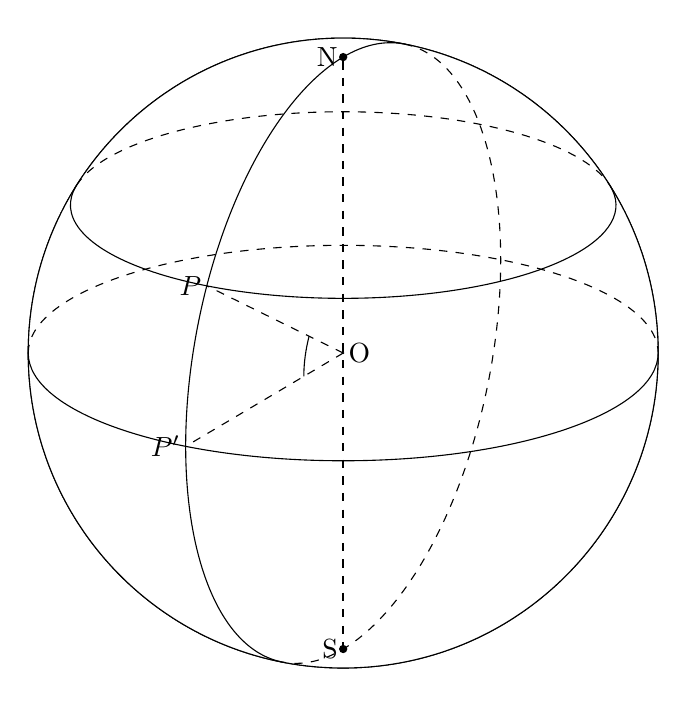
\begin{tikzpicture} % "THE GLOBE" showcase
\def\R{4 } % sphere radius
\def\angEl{20} % elevation angle
\def\angAz{-20} % azimuth angle
\filldraw[ball color=white] (0,0) circle (\R);
\filldraw[fill=white] (0,0) circle (\R);

\foreach \t in {0,30} { \DrawLatitudeCircle[\R]{\t} }
\foreach \t in {-120} { \DrawLongitudeCircle[\R]{\t} }


\pgfmathsetmacro\H{\R*cos(\angEl)} % distance to north pole
\coordinate (O) at (0,0);
\node[circle,draw,black,scale=0.3] at (0,0) {};
\draw[right] node at (0,0){O};
\coordinate[mark coordinate] (N) at (0,\H);
\draw[left] node at (0,\H){N};
\coordinate[mark coordinate] (S) at (0,-\H);
\draw[left] node at (0,-\H){S};
\draw[thick, dashed, black](N)--(S);

\NewLatitudePlane[planeP]{\R}{\angEl}{30};
\path[planeP] (-120:\R) coordinate (P);
\draw[left] node at (P){$P$};

\NewLatitudePlane[equator]{\R}{\angEl}{00};
\path[equator] (-120:\R) coordinate (Pprime);
\draw[left] node at (Pprime){$P'$};

\draw[-,dashed] (O)--(P);
\draw[-,dashed] (O)--(Pprime);

\LongitudePlane[angle]{\angEl}{-120};
\draw[angle,-] (0:1) arc (0:30:1);

\end{tikzpicture}

\end{document}